% Options for packages loaded elsewhere
\PassOptionsToPackage{unicode}{hyperref}
\PassOptionsToPackage{hyphens}{url}
%
\documentclass[
  14pt,
]{extarticle}
\usepackage{amsmath,amssymb}
\usepackage{lmodern}
\usepackage{iftex}
\ifPDFTeX
  \usepackage[T1]{fontenc}
  \usepackage[utf8]{inputenc}
  \usepackage{textcomp} % provide euro and other symbols
\else % if luatex or xetex
  \usepackage{unicode-math}
  \defaultfontfeatures{Scale=MatchLowercase}
  \defaultfontfeatures[\rmfamily]{Ligatures=TeX,Scale=1}
\fi
% Use upquote if available, for straight quotes in verbatim environments
\IfFileExists{upquote.sty}{\usepackage{upquote}}{}
\IfFileExists{microtype.sty}{% use microtype if available
  \usepackage[]{microtype}
  \UseMicrotypeSet[protrusion]{basicmath} % disable protrusion for tt fonts
}{}
\makeatletter
\@ifundefined{KOMAClassName}{% if non-KOMA class
  \IfFileExists{parskip.sty}{%
    \usepackage{parskip}
  }{% else
    \setlength{\parindent}{0pt}
    \setlength{\parskip}{6pt plus 2pt minus 1pt}}
}{% if KOMA class
  \KOMAoptions{parskip=half}}
\makeatother
\usepackage{xcolor}
\usepackage[margin=1.5cm,bottom=2.5cm,top=2.5cm,headsep=0cm,headheight=5cm]{geometry}
\usepackage{graphicx}
\makeatletter
\def\maxwidth{\ifdim\Gin@nat@width>\linewidth\linewidth\else\Gin@nat@width\fi}
\def\maxheight{\ifdim\Gin@nat@height>\textheight\textheight\else\Gin@nat@height\fi}
\makeatother
% Scale images if necessary, so that they will not overflow the page
% margins by default, and it is still possible to overwrite the defaults
% using explicit options in \includegraphics[width, height, ...]{}
\setkeys{Gin}{width=\maxwidth,height=\maxheight,keepaspectratio}
% Set default figure placement to htbp
\makeatletter
\def\fps@figure{htbp}
\makeatother
\setlength{\emergencystretch}{3em} % prevent overfull lines
\providecommand{\tightlist}{%
  \setlength{\itemsep}{0pt}\setlength{\parskip}{0pt}}
\setcounter{secnumdepth}{-\maxdimen} % remove section numbering

\usepackage{gensymb}
\usepackage{mhchem}
\usepackage{tcolorbox}
\usepackage{fancyhdr}
\usepackage{graphicx}
\usepackage{titling}
\ifLuaTeX
  \usepackage{selnolig}  % disable illegal ligatures
\fi
\IfFileExists{bookmark.sty}{\usepackage{bookmark}}{\usepackage{hyperref}}
\IfFileExists{xurl.sty}{\usepackage{xurl}}{} % add URL line breaks if available
\urlstyle{same} % disable monospaced font for URLs
\hypersetup{
  pdftitle={Laws of Chemical Combination},
  hidelinks,
  pdfcreator={LaTeX via pandoc}}

\title{\textbf{Laws of Chemical Combination}}
\usepackage{etoolbox}
\makeatletter
\providecommand{\subtitle}[1]{% add subtitle to \maketitle
  \apptocmd{\@title}{\par {\large #1 \par}}{}{}
}
\makeatother
\subtitle{\textbf{Unit 1:} Some Basic Concepts in Chemistry}
\author{}
\date{}


\pagestyle{fancy}
% \graphicspath{{./images/}}
\fancyhead[C]{
\includegraphics[width=2cm]{./images/fplogo}}
\fancyhead[L]{JEE Chemistry\\~\\}
\fancyhead[R]{\thetitle{}\\~\\}
\renewcommand{\headrulewidth}{0pt}
\renewcommand{\footrulewidth}{2pt}
\newtcolorbox{myquote}{colback=gray!25, colframe=gray!75!black}
\renewenvironment{quote}{\begin{myquote}}{\end{myquote}}
% \let\OldRule\rule
% \renewcommand{\rule}[2]{\OldRule{\linewidth}{#2}}
\newcommand{\ud}[2]{\underset{\text{#2}}{\ce{#1}}}

\begin{document}
\maketitle
\thispagestyle{fancy}

\hypertarget{law-of-conservation-of-mass-lavoisier}{%
\section{Law of Conservation of Mass
(Lavoisier)}\label{law-of-conservation-of-mass-lavoisier}}

\textbf{In a chemical reaction, mass is neither created nor destroyed.
Only rearrangement of atoms takes place.} \[
\text{Sum of mass of reactants} = 
\text{Sum of mass of products}
\]

Example: When \({4.2~\mathrm{g}}\) \(\ce{NaHCO3}\) is added to a
solution of \(\ce{CH3COOH}\) weighing \({10.0~\mathrm{g}}\), it is
observed that \({2.2~\mathrm{g}}\) \(\ce{CO2}\) is released into
atmosphere. The residue is found to weight \({12.0~\mathrm{g}}\). \[
\ce{\ud{NaHCO3}{4.2g} + \ud{CH3COOH}{10.0g} -> \ud{CH3COONa + H2O}{12g} +\ud{CO2}{2.2g}}
\] \[\text{Mass of Reactants}=4.2 + 10.0 = {14.2~\mathrm{g}}\]
\[\text{Mass of Products}=12 + 2.2 = {14.2~\mathrm{g}}\] Hence, the mass
is conserved.

\begin{quote}
In nuclear reactions, the mass is not conserved. Here, the mass gets
converted to energy, as explained by Einstein. Therefore, the law is
more accurately known as the Law of Conservation of Mass and Energy.
\end{quote}

\hypertarget{law-of-constant-proportions-joseph-proust}{%
\section{Law of Constant Proportions (Joseph
Proust)}\label{law-of-constant-proportions-joseph-proust}}

\textbf{For a specific compound, the constituent elements of a compound
are always in a constant proportion, irrespective of its source.}

Example: Water (\(\ce{H2O}\)) always has hydrogen and oxygen present in
\(1:8\) mass ratio, whether it is tap water, sea water or distilled
water.

\hypertarget{law-of-multiple-proportions-dalton}{%
\section{Law of Multiple Proportions
(Dalton)}\label{law-of-multiple-proportions-dalton}}

\textbf{If two elements form more than one compound, then the different
masses of one element, which combine with the fixed mass of the other
element, bear a simple whole number ratio.}

Example: \[\ce{H2O} \rightarrow \mathrm{H} - 2g ~~ \mathrm{O} - 16g\]
\[\ce{H2O2}\rightarrow \mathrm{H} - 2g ~~ \mathrm{O} - 32g\] Here,
masses of oxygen bears a simple whole number ratio - \(16:32=1:2\)

\begin{quote}
\begin{itemize}
\tightlist
\item
  These laws is not applicable in case of compounds formed by different
  isotopes of the same element.
\end{itemize}
\end{quote}

\hypertarget{law-of-reciprocal-proportions-richter}{%
\section{Law of Reciprocal Proportions
(Richter)}\label{law-of-reciprocal-proportions-richter}}

\textbf{The ratio of the weights of two elements A and B which combine
separately with a fixed weight of the third element C is either the same
or some simple multiple of the ratio of the weights in which A and B
combine directly with each other.}

Example:

\begin{center}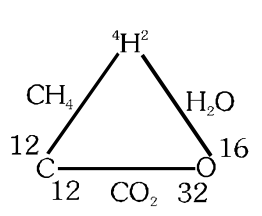
\includegraphics[width=1.04167in,height=\textheight]{./images/2022-06-22-23-05-22.png}\end{center}

The elements C and O combine separately with the third element H to form
\(\ce{CH4}\) and \(\ce{H2O}\) and they combine directly with each other
to form CO2. - In \(\ce{CH4}\), 4 H combines with 12 C by mass. - In
\(\ce{H2O}\), 2 H combines with 16 O by mass, or 4 H combines with 32 O
by mass. - Thus, a fixed weight of H (4 parts) reacts with C and O in
the ratio \(12:32=3:8\).

Now, in \(\ce{CO2}\), 12 C combines with 32 O. This ratio is same as the
one derived above. Hence, the law holds true.

\hypertarget{law-of-combining-volumes-gay-lussac}{%
\section{Law of Combining Volumes (Gay
Lussac)}\label{law-of-combining-volumes-gay-lussac}}

\textbf{When gases react together, they do so in a simple whole number
ratio by volume to one another and the products, at S.T.P.}

Example:

\begin{center}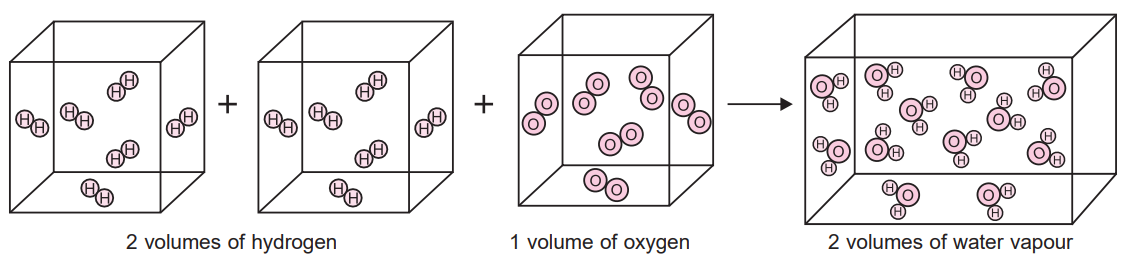
\includegraphics{./images/2022-06-22-23-18-27.png}\end{center}

It has been found, that 2 volumes of hydrogen react with 1 volume of
oxygen to produce 2 volumes of water vapour. Thus, the volumes of these
gases bear a simple whole number ratio of \(2:1:2\).

\begin{quote}
It might be somewhat counterintuitive to understand that 2 volumes of H
and 1 volume of O forms only 2 volumes and not 3 (2+1) volumes. This is
because of the fact that gases don't have a fixed volume, and unlike
mass, volume is not conserved. Therefore, volumes cannot be added and
subtracted like mass.

The reason due to which this above reaction takes place in this volume
ratio will be explained later in this unit.
\end{quote}

\hypertarget{avogadros-law-avogadro}{%
\section{Avogadro's Law (Avogadro)}\label{avogadros-law-avogadro}}

\textbf{Under similar conditions of temperature and pressure, equal
volumes of all gases contain equal number of molecules.}

\[\text{V}\propto\text{N}\]

Example: 1 L of Hydrogen gas, 1 L of Oxygen gas and 1 L of Chlorine gas
all have the same number of molecules.

\begin{quote}
We can relate Avogadro's Law to Gay Lussac's Law to understand the
relations between volume and number of molecules.
\[\ce{2H2 + O2 -> 2H2O}\] Here, 2 molecules of hydrogen react with 1
molecule of oxygen and form 2 molecules of water.\\
This can also be written as 2n molecules of H react with n molecules of
O to form 2n molecules of \(\ce{H2O}\).\\
From Avogadro's Law, we can say that 2n molecules refer to 2 volumes of
the gas, and n molecules refer to 1 volume of the gas. Thus, 2 volumes
of hydrogen react with 1 volume of oxygen to produce 2 volumes of water
vapour. This result is in agreement to the Gay Lussac's Law.
\end{quote}

\begin{center}\rule{0.5\linewidth}{0.5pt}\end{center}

\hypertarget{questions}{%
\section{Questions}\label{questions}}

\begin{enumerate}
\def\labelenumi{\arabic{enumi}.}
\item
  If 6.3 g of \(\ce{NaHCO3}\) are added to 15.0 g \(\ce{CH3COOH}\)
  solution, the residue is found to weigh 18.0 g. What is the mass of
  \(\ce{CO2}\) released in the reaction?

  \begin{enumerate}
  \def\labelenumii{(\Alph{enumii})}
  \tightlist
  \item
    4.5 g
  \item
    3.3 g
  \item
    2.6 g
  \item
    2.8 g
  \end{enumerate}
\item
  3 g of a hydrocarbon on combustion in excess of oxygen produces 8.8 g
  of \(\ce{CO2}\) and 5.4 g of \(\ce{H2O}\). The data illustrates the
  law of: \textbf{{[}JEE 2010{]}}

  \begin{enumerate}
  \def\labelenumii{(\Alph{enumii})}
  \tightlist
  \item
    conservation of mass
  \item
    multiple proportions
  \item
    constant proportions
  \item
    none of these
  \end{enumerate}
\item
  One of the statements of Dalton's atomic theory is given below.\\
  ``Compounds are formed when atoms of different elements combine in a
  fixed ratio.''\\
  Which of the following laws is not related to this statement?
  (Multiple Correct Options)

  \begin{enumerate}
  \def\labelenumii{(\Alph{enumii})}
  \tightlist
  \item
    Law of conservation of mass
  \item
    Law of definite proportions
  \item
    Law of multiple proportions
  \item
    Avogadro's Law
  \end{enumerate}
\item
  Two aqueous solutions X and Y containing 0.585 g of sodium chloride
  and 1.70 g of silver nitrate respectively were mized. The weight of
  silver chloride formed was found to be 1.432 g and 0.853 g
  \(\ce{NaNO3}\) was obtained. Show that these observations confirm the
  law of chemical conservation of mass.
\item
  Iron forms two oxides. In the first oxide, 56g Fe reacts with 16g
  \(\ce{O2}\) and in the second oxide 112g Fe reacts with 48g
  \(\ce{O2}\). This data satisfies the law of

  \begin{enumerate}
  \def\labelenumii{(\Alph{enumii})}
  \tightlist
  \item
    Conservation of Mass
  \item
    Reciprocal Proportions
  \item
    Multiple Proportion
  \item
    Combining Volumes
  \end{enumerate}
\end{enumerate}

Answers\footnote{Answers: 1-(B) 2-(A) 3-(A,D) 5-(C)} are given below.

\end{document}